\chapter{Persistierung} % (fold)
\label{cha:persistierung}

In den vorangegangen drei Kapiteln wurde die Umsetzung des eigentlichen Werkzeugs beschrieben. Neben der Unterstützung des Modellierungsvorgangs ist aber auch die persistente Speicherung der erstellten Modelle zum Zwecke der Weiterverarbeitung ein hier zu beleuchtender Aspekt. Auf die Persistierung wirken vor allem zwei der in Kapitel XY identifzierten Anforderungen ein. Zum ersten ist die Nachvollziehbarkeit des Modellierungsvorganges sicherzustellen -- dies gilt nicht nur während des Vorgangs selbst, sondern auch danach. Dementsprechend ist sämtliche Information zu persistieren, die zur Wiederherstellung nicht nur des Modells selbst sondern auch der gesamten Modellierungshistorie notwendig ist. Zum zweiten hat die Forderung nach semantischer Offenheit bei der Modellierung auch unmittelbare Auswirkungen auf die Persistierung. Neben dem Modell selbst muss aufgrund dieser Anforderung auch die Bedeutung der verwendeten Modellierungselemente miterfasst und persistiert werden, so dass diese bei der Weiterverarbeitung der Modelle verwendet werden kann.

In diesem Kapitel werden nun aufgrund der eben genannten Forderungen technologische Ansätze identifiziert, beschrieben und schließlich hinsichtlich ihrer Eignung für den konkreten Einsatz beurteilt. Der ausgewählte Ansatz wird im darauf folgenden Abschnitt konzeptuell beschrieben. Die Abbildung der Modelle und der ebenfalls zu persistierenden zusätzlichen Information in ein geeignetes Datenmodell ist Gegenstand des darauf folgenden Abschnitts. Schließlich wird die konkrete technische Umsetzung der Persistierung dargelegt und die dazu notwendigen Software-Module im Detail beschrieben.
 
\section{Möglichkeiten der Persistenzsicherung} % (fold)
\label{sec:möglichkeiten_der_persistenzsicherung}

\begin{itemize}
	\item Serialisierung von Java-Objekten
	\item Relationale Datenbanken
	\item XML Topic Maps
\end{itemize}

% section möglichkeiten_der_persistenzsicherung (end)

\section{Topic Maps} % (fold)
\label{sec:topic_maps}

Topic Maps \citep{TMDM08} sind wie bereits in Abschnitt XY beschrieben ein Mittel zur Abbildung von semantischen Netzen. In Topic Maps können beliebige Daten strukutriert aufbereitet und zueinander in Beziehung gesetzt werden. Die Art der zu repräsentierenden Daten ist dabei irrelvant, eine Topic Map trifft keine Aussage über ein den repräsentierten Daten zugrundeliegendes Begriffsystem (sie ist „ontology-agnostic“ \citep{Vatant04}).

Historisch stammen Topic Maps aus dem Bereich der technischen Repräsentation von Thesauri und Indizes \citep{Pepper00} \citep{Rath03}. Aus diesen Bereichen motivieren sich auch die Bausteine einer Topic Map, wenngleich der Verwendung durch diesen Ursprung nicht eingeschränkt wird. Die grundlegenden Elemente einer Topic Map sind „Topics“, „Associations“ und „Occurrences“ (siehe Abbildung \ref{fig:img_Persistenz_TMBasic}). 

\begin{figure}[htbp]
	\centering
		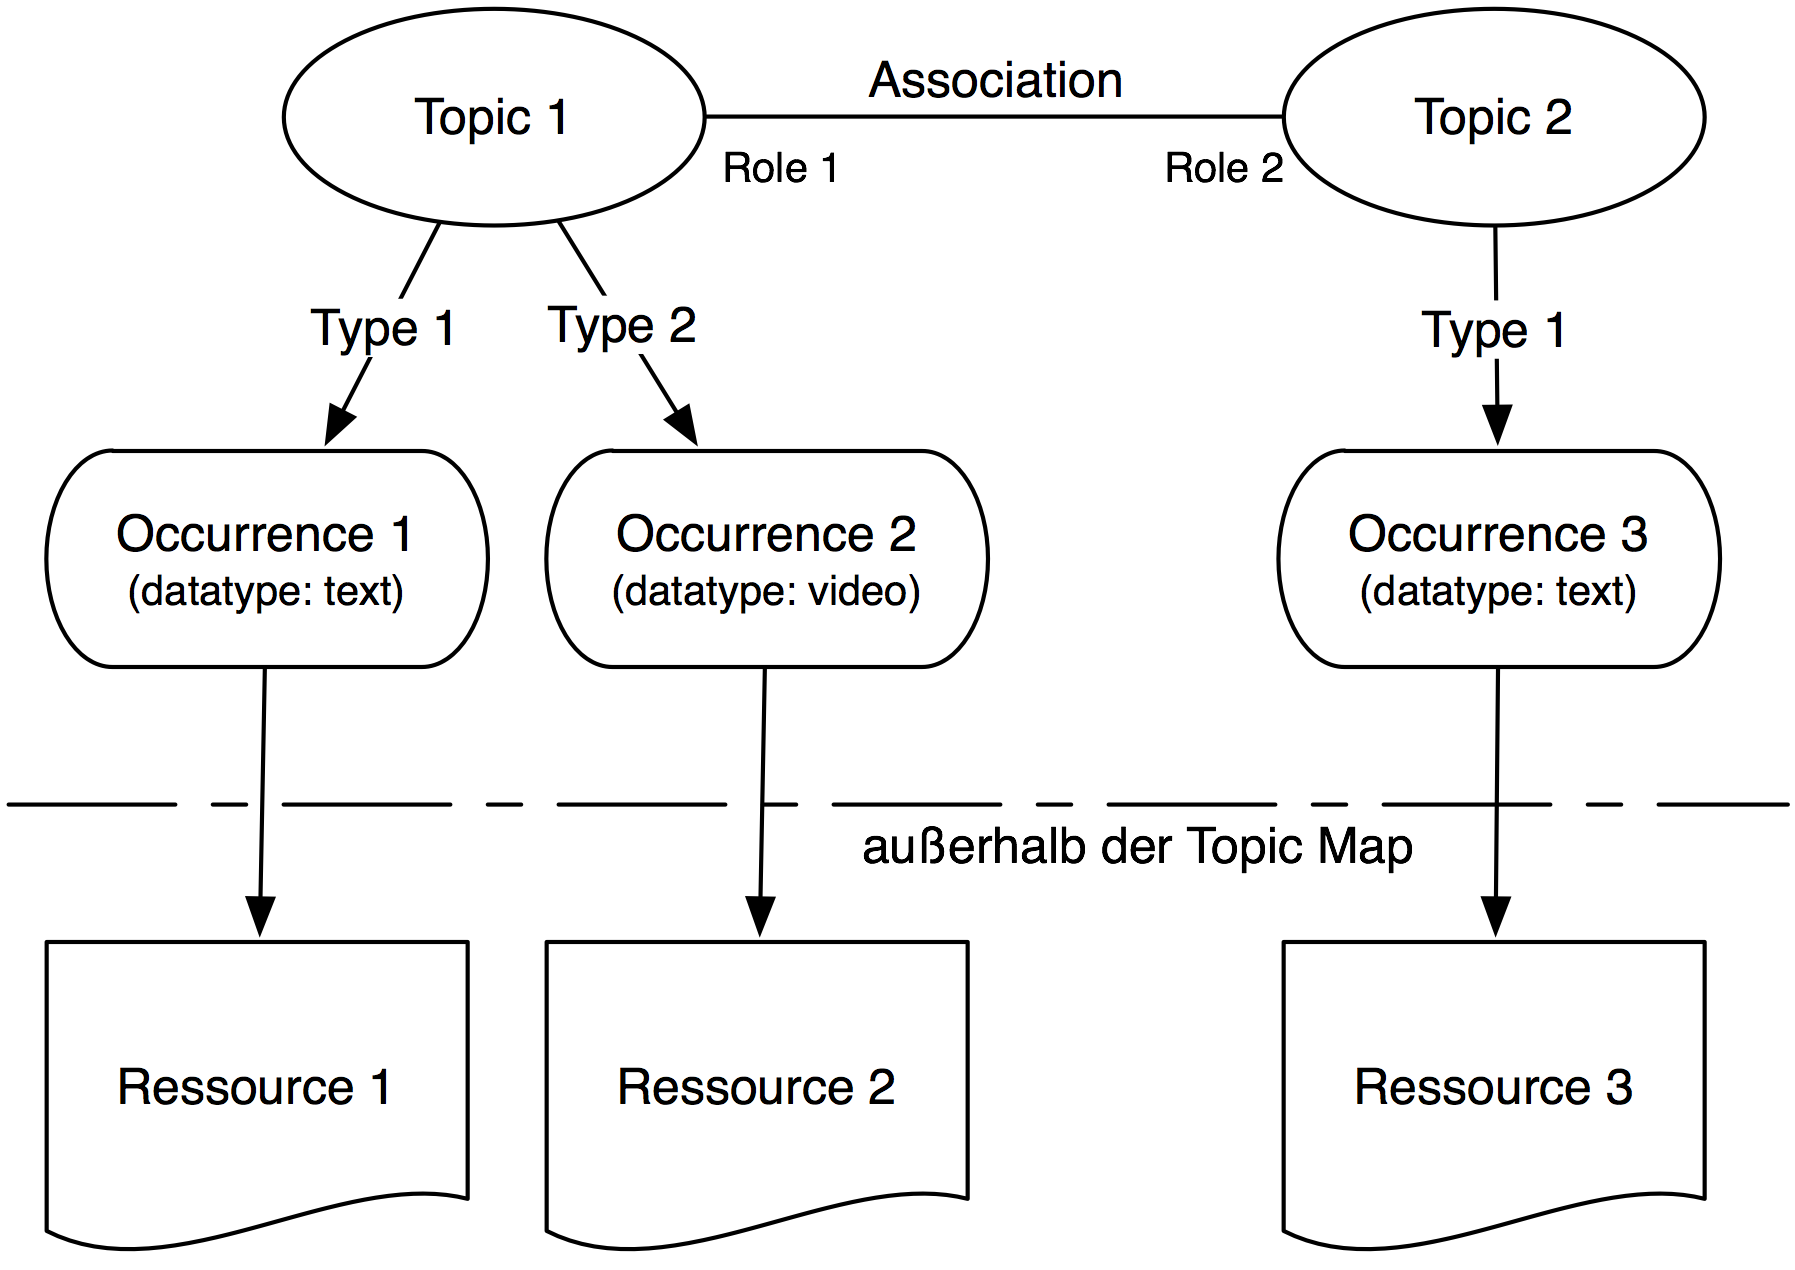
\includegraphics[width=10cm]{img/Persistenz/TMBasic.png}
	\caption{Grundlegende Elemente einer Topic Map}
	\label{fig:img_Persistenz_TMBasic}
\end{figure}

„Topics“ sind stellen Begriffe dar und bilden die Knoten des semantischen Netzes. Ein Topic kann beliebige Information darstellen, repräsentiert aber immer genau ein Phänomen der realen Welt (d.h. zu einem Topic muss es eine Entsprechung außerhalb der Topic Maps geben, die beobachtbar oder beschreibbar ist und auf die die modellierende Person Bezug nehmen will \footnote{„A subject can be anything whatsoever, regardless of whether it exists or has any other specific characteristics, about which anything whatsoever may be asserted by any means whatsoever. In particular, it is anything about which the creator of a topic map chooses to discourse.“ \citep[][S.8]{TMDM08}}). Eine Topic Map ist damit im Sinne von \citet{Stachowiak73} ein diagrammatisches Modell, das einen bestimmten, für den Modellersteller relevanten Ausschnitt der Realität abbildet.

"Associations" bilden die Beziehungen zwischen Topics ab und stellen damit die Kanten des semantischen Netzes dar. Eine Association verknüpft Topics semantisch miteinander und kann frei mit Bedeutung belegt werden. Die Art der Beziehungen ist also nicht festgelegt und wird wie die Bedeutung der Topics frei gewählt werden. Topics und Associations decken historisch den Bereich der Darstellung von Thesauri ab, in denen Begriffe definiert und zueinanden in Beziehung gesetzt werden. 

Der zweite historische Ursprung von Topic Maps, die Indizes, werden durch das Konstrukt der "Occurences" abgedeckt. Occurences ("Auftreten") sind Referenzen aus der Topic Map in die reale Welt. Sie setzen die Topics einer Topic Map in Bezug zu beliebiger referenzierbarer Information (z.B. Dokumente). Im Kontext der eben genannten Indizes, kann eine Topic Map als der mit Querverweisen versehene Index eines Buches verstanden werden, in dem durch die Angabe von Seitenzahlen auf den Text des Buches verwiesen wird. Diese Verweise durch Angabe der Seitenzahlen sind in diesem Zusammenhang die Occurrences.

Die Ansammlung von durch Associations verknüpften und mit Occurrences versehenen Topics bilden eine Topic Map. Darüber hinaus kann in Topic Maps jedoch noch weiterführende Information repräsentiert werden (siehe Abbildung \ref{fig:img_Persistenz_TMFull}), die Gegenstand der folgenden Abschnitte sein werden.

\begin{figure}[htbp]
	\centering
		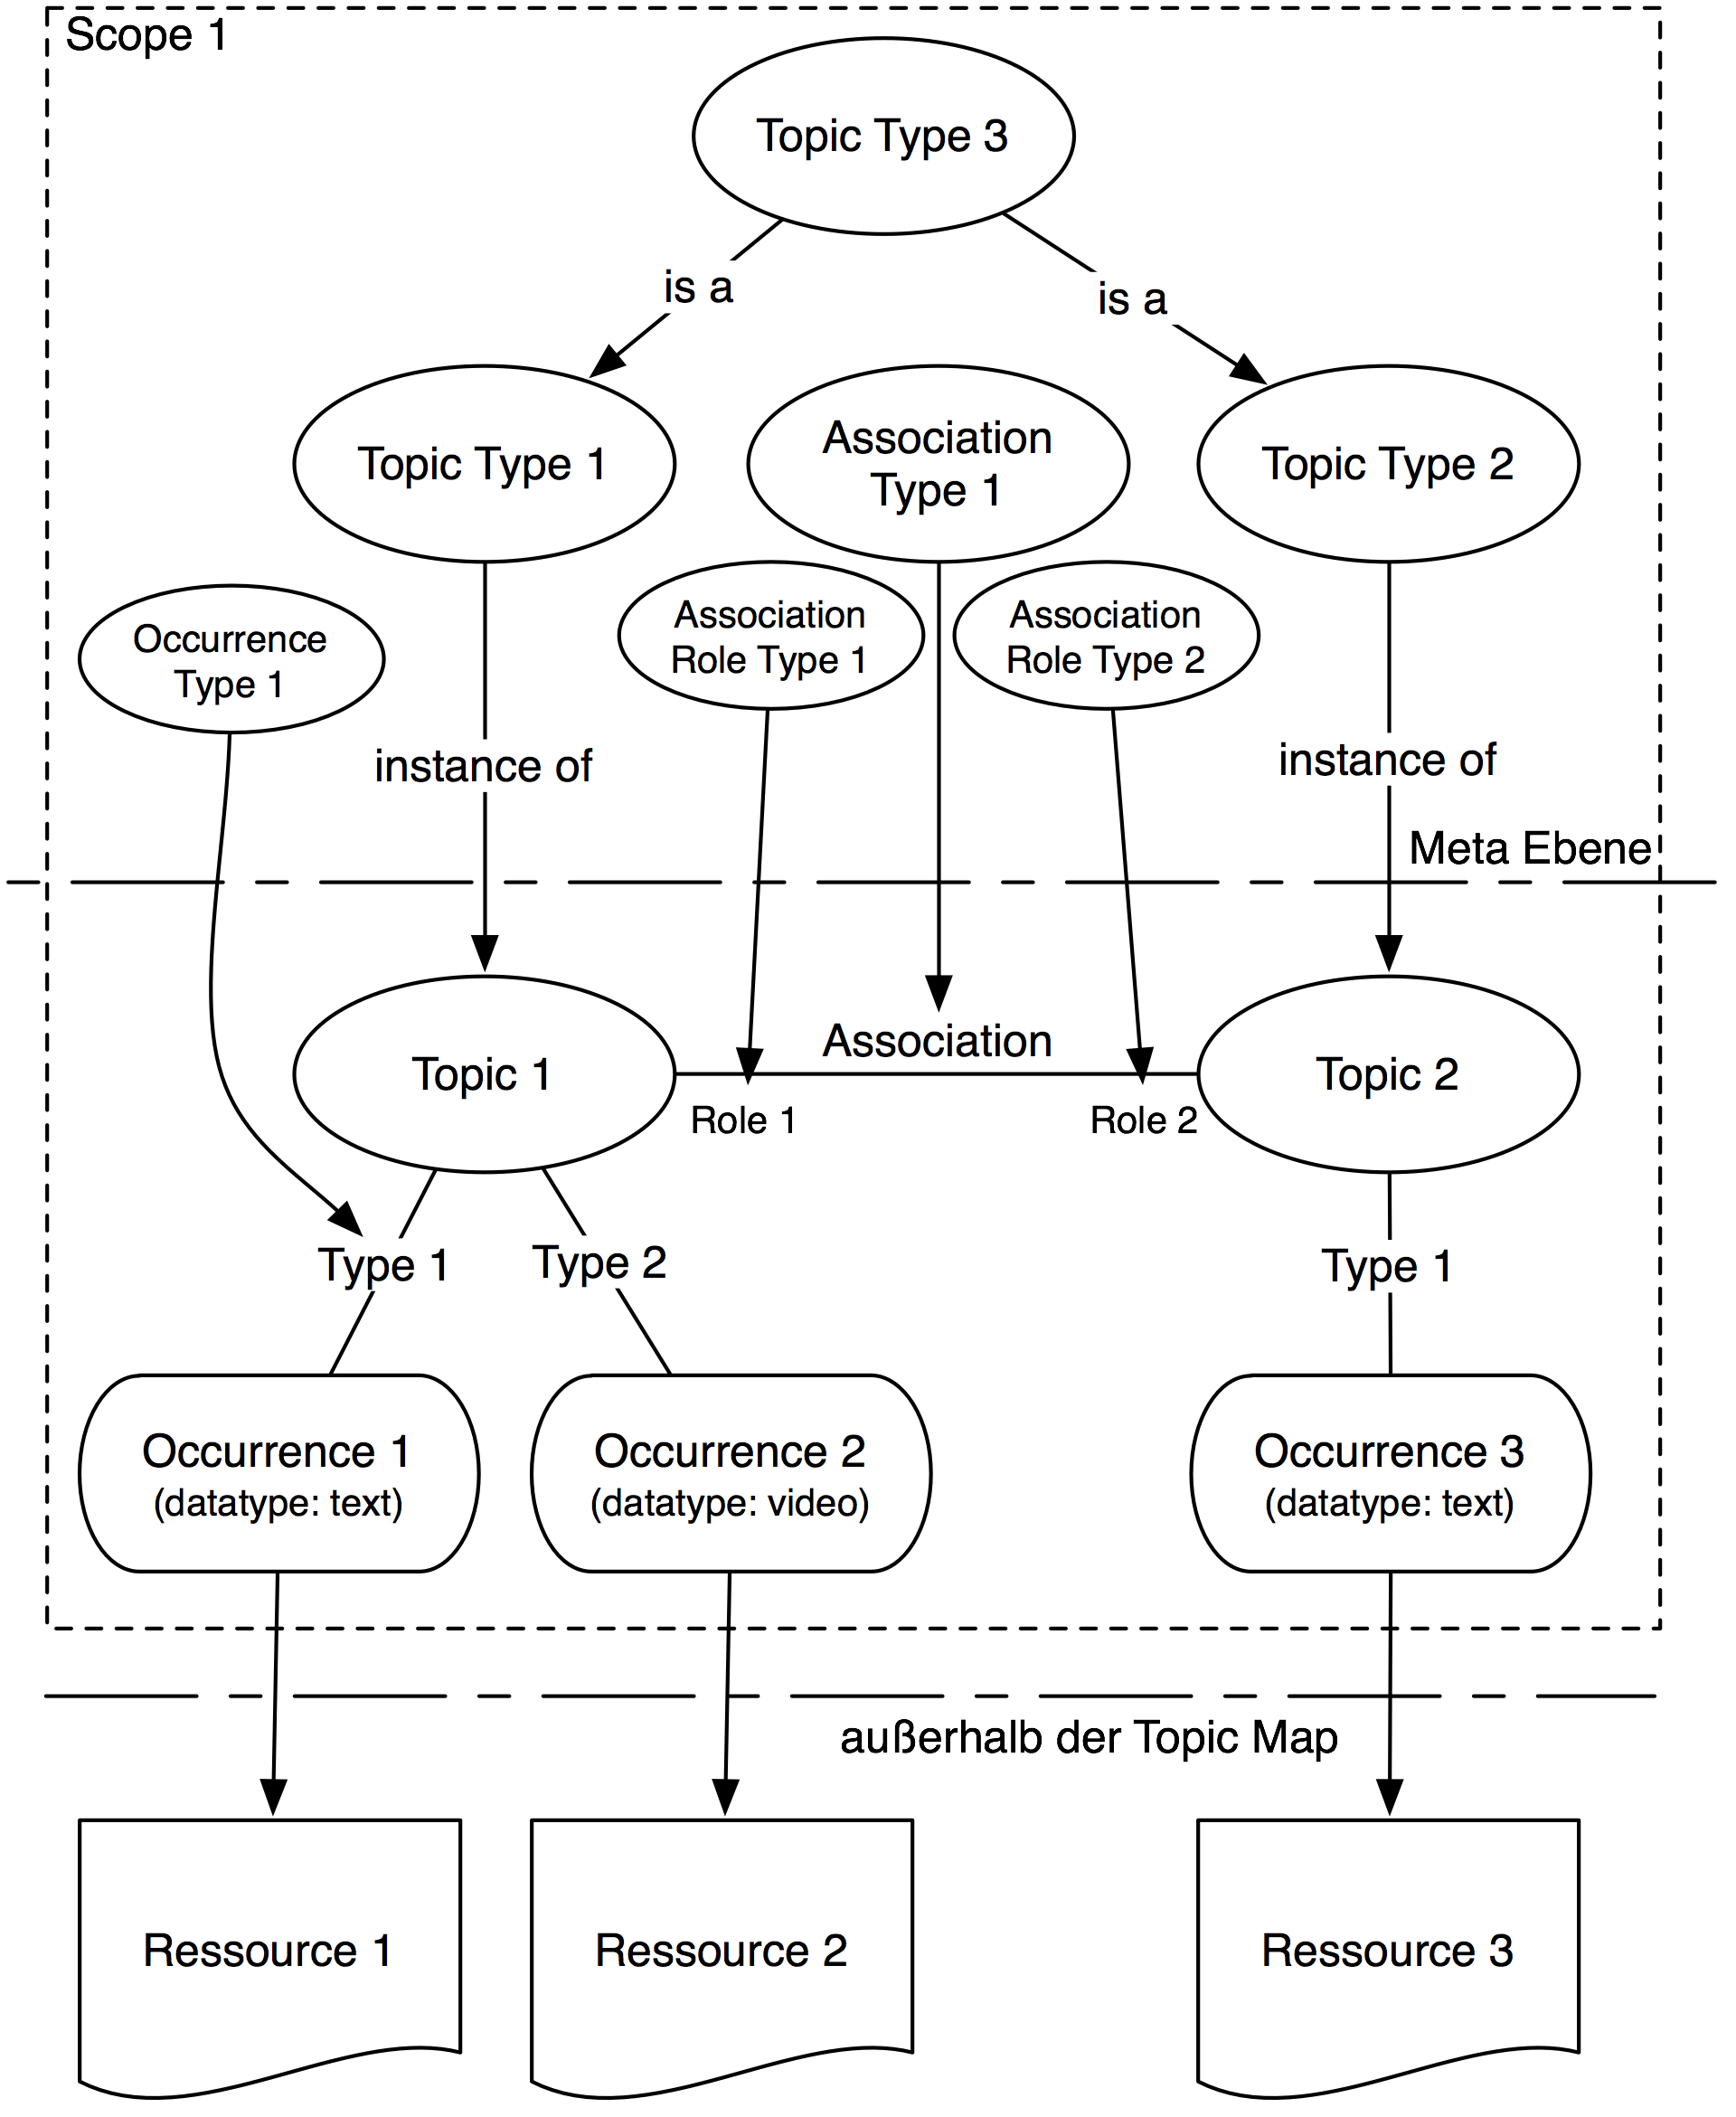
\includegraphics[width=10cm]{img/Persistenz/TMFull.png}
	\caption{Umfassende Darstellung der Elemente einer Topic Map}
	\label{fig:img_Persistenz_TMFull}
\end{figure}

\subsection{Topics, Subjects, Topic Names und Variants} % (fold)
\label{sub:topics_subjects_topic_names_und_variants}

Wie oben bereits beschrieben, repräsentiert ein Topic ein Phänomen der realen Welt in einer Topic Map. Dieses Phänomen der realen Welt, das durch das Topic repräsentiert wird, wird als „Subject“ bezeichnet. In einer Topic Map darf es zu einem Subject nur exakt ein Topic geben, umgekehrt kann ein Topic auch nicht mehrere Subjects repräsentieren, die Zuordnung zwischen Subject und Topic ist also eineindeutig (bijektiv). Im Topic wird dazu exakt ein „Subject Identifier“ registriert, der auf eine Informationsressource verweist, die das Subject für Menschen eindeutig identifizierbar macht (diese Ressource wird als „Subject Indicator“ bezeichnet). Zusätzlich kann ein „Subject Locator“ angegeben werden, der auf das tatsächlich in der realen Welt vorhandene Subject verweist. In Abgrenzung dazu kann es bei der anderen Brücke zwischen realer Welt und Topic Map, den Occurrences, für jeder Topic beliebig viele Zuordnungen geben. Eine Occurrence referenziert auch auf die reale Welt, zeigt aber dort nicht auf das Subject selbst, sondern auf ein dieses Subject beschreibendes Objekt in der realen Welt. Beispielhaft ist dazu in Abbildung \ref{fig:img_Persistenz_SubjectVsOccurrence} dieser Zusammenhang anhand des Topics „Tasse“ dargestellt. Ein anderes Beispiel ist ein Topic „London“, das als Subject die reale Stadt London repräsentiert und dem eine Occurrence zugeordnet werden könnte, die auf eine Landkarte (als in der Realität vorhandene Beschreibung der realen Stadt London) referenziert.

\begin{figure}[htbp]
	\centering
		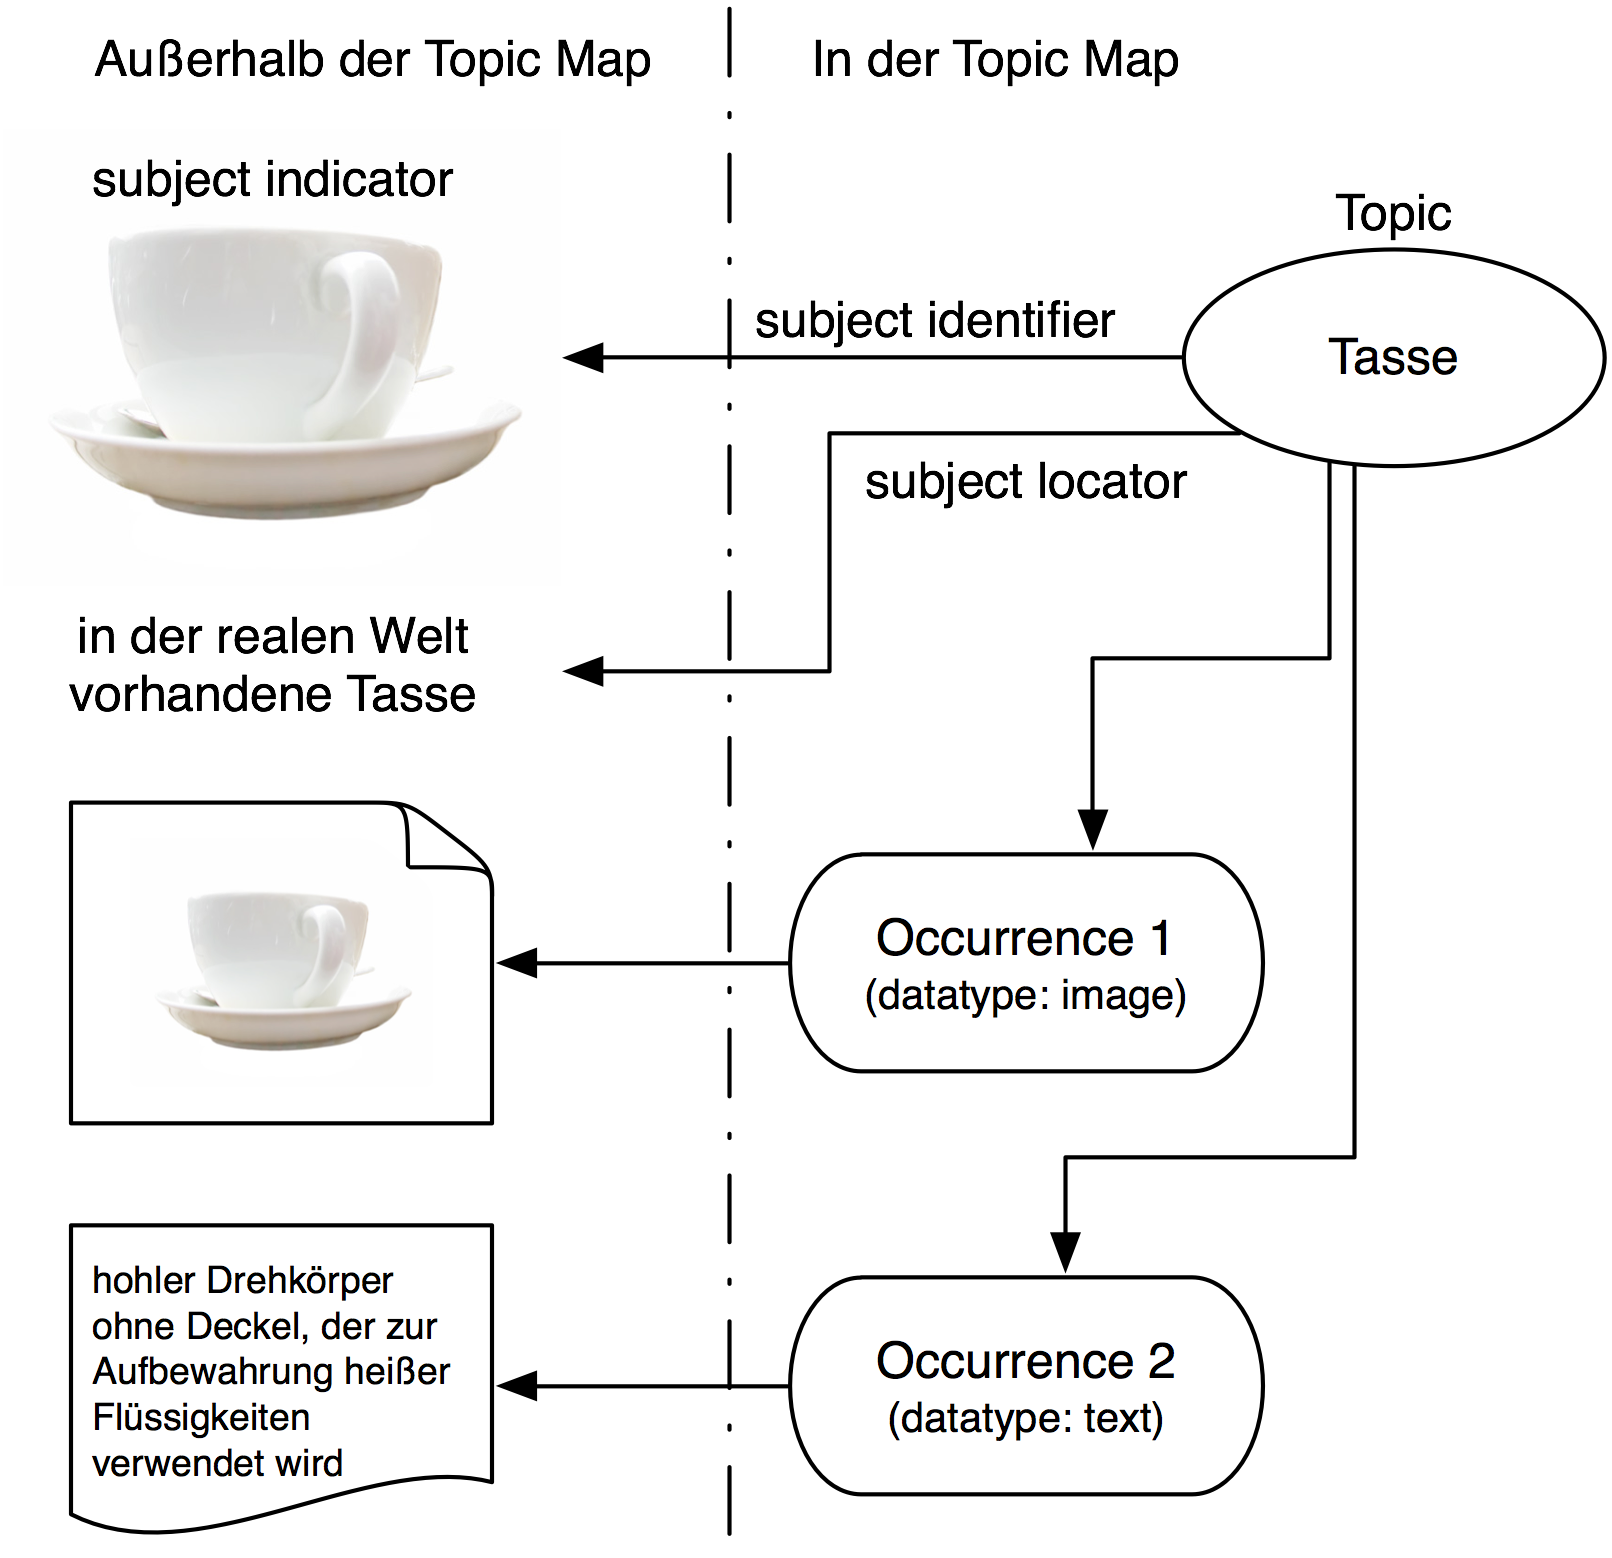
\includegraphics[width=10cm]{img/Persistenz/SubjectVsOccurrence.png}
	\caption{Abgrenzung zwischen Subject und Occurrence in Topic Maps}
	\label{fig:img_Persistenz_SubjectVsOccurrence}
\end{figure}

Bislang wurde vereinfacht ein Topic immer mit einem direkt zugeordneten Namen dargestellt. In einer Topic Map besitzt ein Topic jedoch keinen eindeutigen Namen. Es wird vielmehr durch seinen Subject Identifier eindeutig gekennzeichnet. Dieser ist jedoch nicht unbedingt für Menschen les- und/oder interpretierbar -- der Subject Identifier hat das Ziel, ein Subject für die Verarbeitung durch Software eindeutig zuordenbar zu machen. Für die Bezeichnung eines Topics in einer für Menschen interpretierbaren Form ist die Verwendung von „Topic Names“ vorgesehen (siehe Abbildung \ref{fig:img_Persistenz_TopicNaming}). Topic Names werden immer textuell angegeben und beschreiben das Subject, das durch das betreffende Topic referenziert wird. Durch einen Topic Name soll das Subject für Menschen erkennbar sein, wobei die Zuordnung nicht notwendigerweise eindeutig sein muss (Beispiel: der Topic Name „Jaguar“ kann ein Fahrzeug oder eine Großkatze bezeichnen und ist dementsprechend ein zulässiger Name für zwei unterschiedliche Topics). Einem Topic können beliebig viele Topic Names zugewiesen werden -- es ist so zum Beispiel möglich, eine mehrsprachige Topic Map zu realisieren, in der zu jedem Topic Topic Names in unterschiedlichen Sprachen angegeben werden. 

\begin{figure}[htbp]
	\centering
		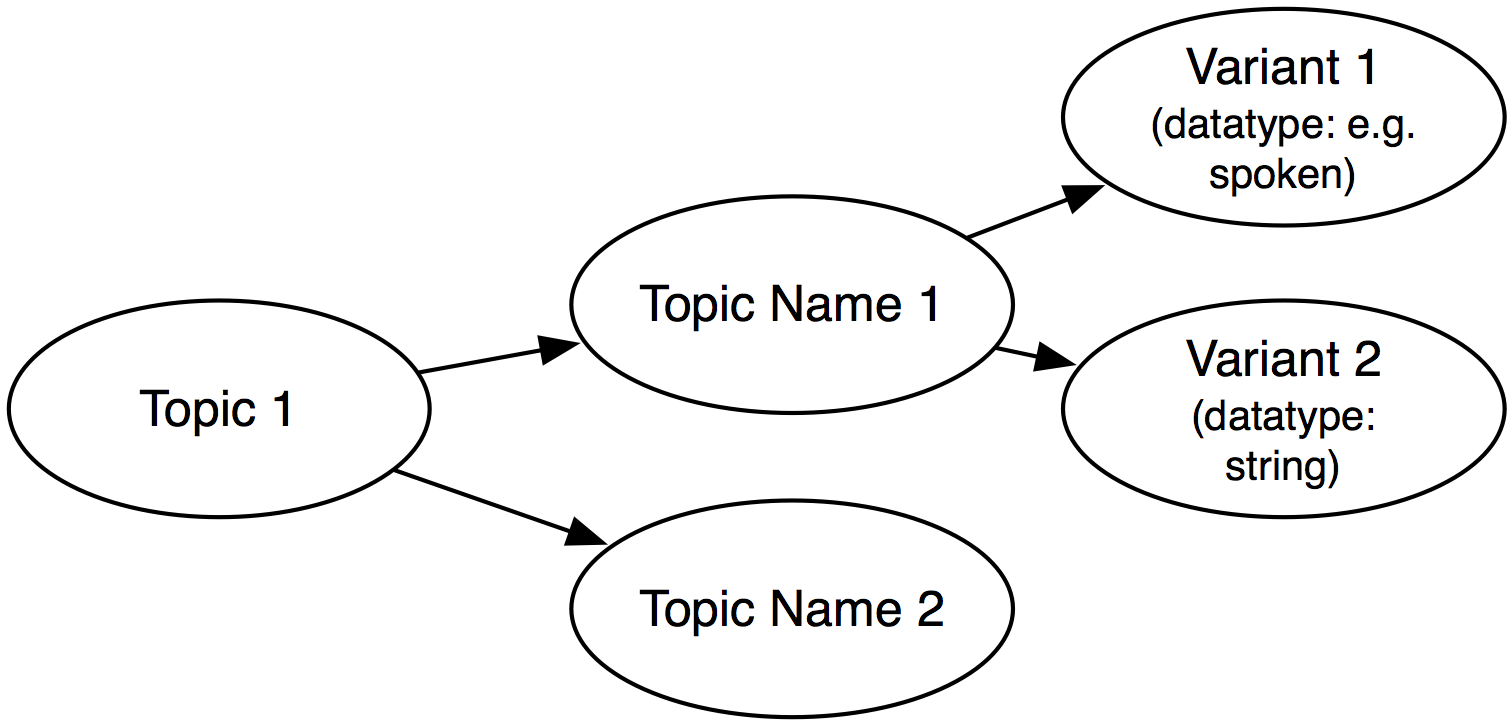
\includegraphics[width=10cm]{img/Persistenz/TopicNaming.png}
	\caption{Benennung von Topics}
	\label{fig:img_Persistenz_TopicNaming}
\end{figure}

Als weitere Detaillierungsstufe können zu jedem Topic Name „Variants“ angegeben werden. Wie durch den Namen angedeutet, handelt es sich dabei um Varianten eines Topic Names, die in bestimmten Zusammenhängen oder für gewisse Anwendungszwecke besser geeignet sein können als der eigentlich Topic Name. Ein Beispiel für eine mögliche Variante ist die Angabe einer gesprochenen Version des Topic Names. Ein weiteres Anwendungsgebiet für Varianten ist die im Standard explizit vorgesehene Angabe eines „Sort Name“ \citep[][S. 18]{TMDM08}, der es erlauben soll, Topic Maps in eine durch diesen Namen vorgegebene Ordnung bringen zu können. Varianten werden durch die Angabe eines dezidiert dafür gewidmeten Topics in deren Scope (siehe Abschnitt \ref{sub:scopes}) als Sort Names gekennzeichnet.

% subsection topics_subjects_topic_names_und_variants (end)

\subsection{Associations und Roles} % (fold)
\label{sub:associations_und_roles}

"Associations" stellen Verbindungen zwischen den einzelnen Topics einer Topic Map her. Associations haben beliebig viele Endpunkte, mindestens jedoch einen (sind also nicht von vorneherein immer binär sondern können auch unär sein oder mehr als zwei Topics verknüpfen). Eine Associations enthält wie ein Topic nicht unmittelbar einen für Menschen lesbaren Namen. Diese wird durch ein Topic festgelegt, das die Kategorie festlegt, der die Association zuzuordnen sind (siehe Abschnitt \ref{sub:metamodellierung_in_topic_maps}). Diesem Topic kann wiederum mindestens ein Topic Name zugeordnet werden, welcher letzendlich die Benennung der Association festlegt.

Associations werden jedoch nicht direkt mit Topics verknüpft. Um ausdrucksstärkere Verknüpfungen realisieren zu können, agieren "Roles" als Verknüpfung zwischen Association und den betreffenden Topics. Roles legen die "Rolle" -- also die Bedeutung -- eines Topics in exakt der betrachteten Association fest. Diese Bedeutung kann generisch sein und zum Beispiel dazu verwendet werden, die per se ungerichteten Associations unabhängig von ihrer konkreten Bedeutung mit einer Richtung zu versehen (zum Beispiel durch die Zuordnung von Roles "Anfang" und "Ende") aber auch um die Beziehung semantisch anzureichern (zum Beispiel durch die Zuordnung von Roles "Veranwortlicher", "Ausführender" und "Prozessschritt" in einer Association "durchzuführen"). Die Anzahl der in einer Association referenzierten Roles gibt damit auch die Kardinalität der Association (also die Anzahl ihrer Endpunkte) an. Aus den konkreten Roles wird dann auf die Topics verwiesen, die diese Roles einnehmen bzw. "spielen" (tatsächlich heißt die betreffende Eigenschaft einer Role "player"). Genau wie Associations werden Roles nicht direkt benannt sondern über ein Topic, das ihre Kategorie bestimmt, mit einer Benennung versehen (Detail wiederum in Abschnitt \ref{sub:metamodellierung_in_topic_maps}).

% subsection associations_und_roles (end)

\subsection{Occurrences und Datatypes} % (fold)
\label{sub:occurrences_und_datatypes}

% subsection occurrences_und_datatypes (end)

\subsection{Metamodellierung in Topic Maps} % (fold)
\label{sub:metamodellierung_in_topic_maps}

Topic Types, Topic Name Types, Association Types und Occurrence Types

\begin{figure}[htbp]
	\centering
		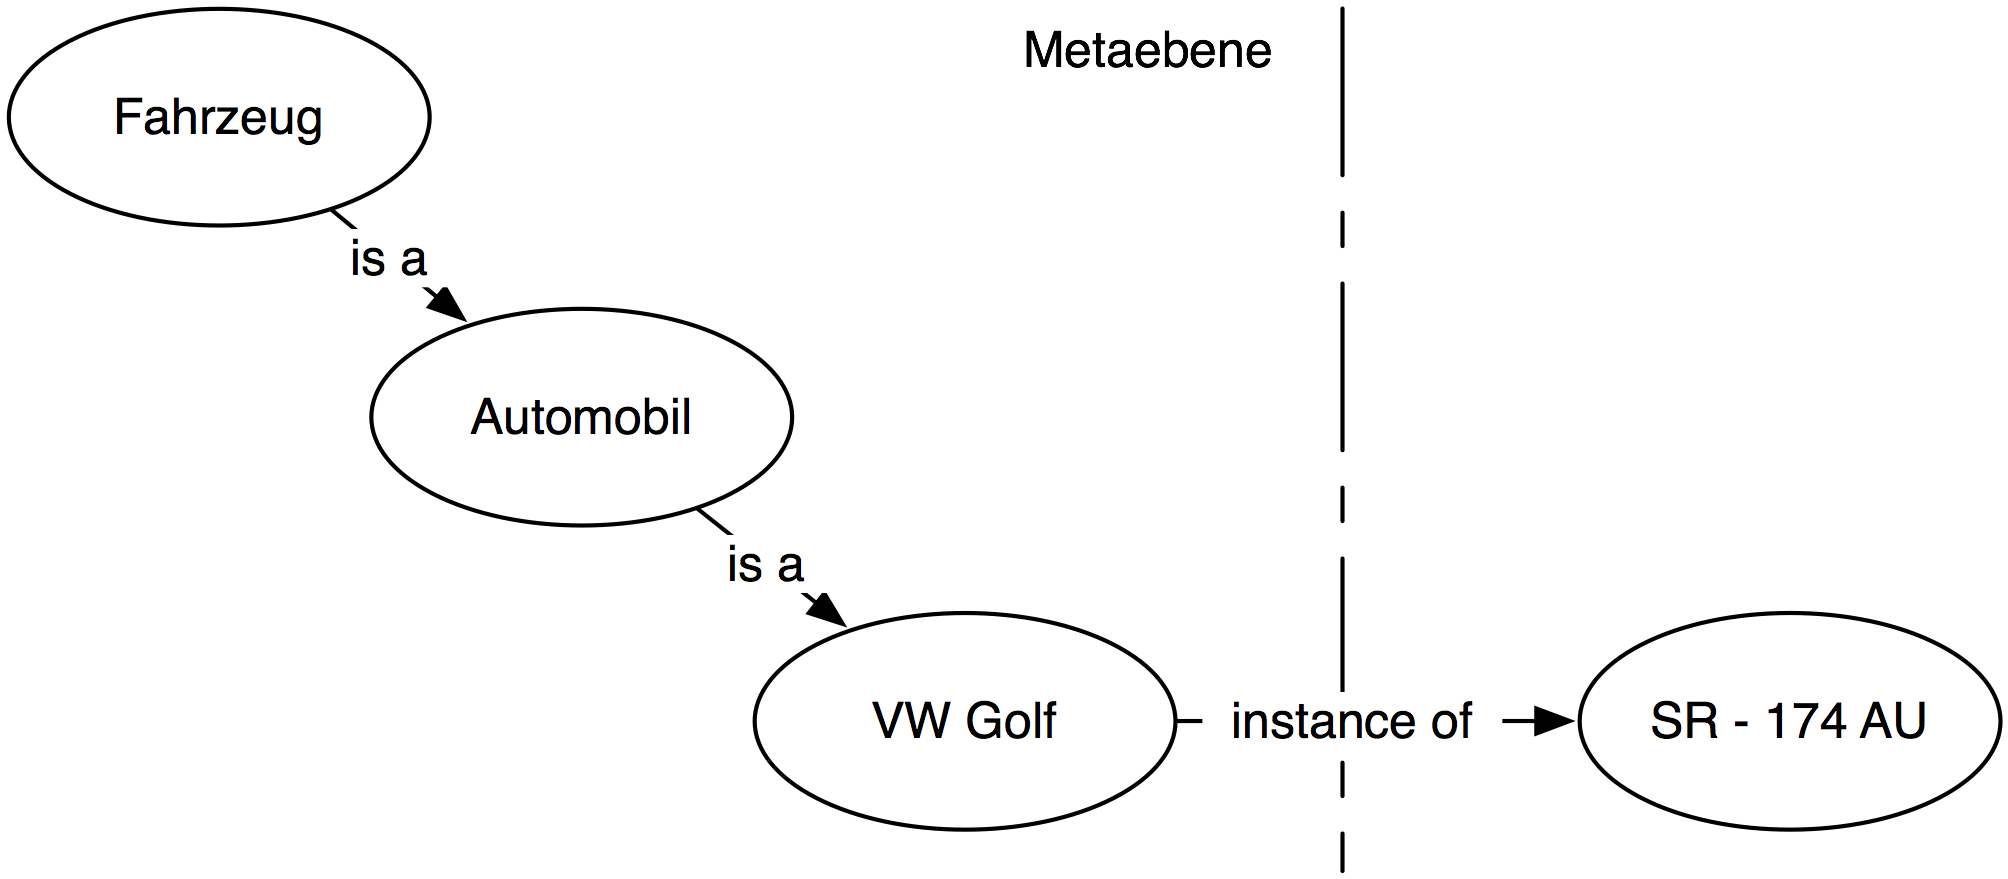
\includegraphics[width=10cm]{img/Persistenz/MetaModelExample.png}
	\caption{Beziehungen in der Metamodellbildung in Topic Maps}
	\label{fig:img_Persistenz_MetaModelExample}
\end{figure}

% subsection metamodellierung_in_topic_maps (end)

\subsection{Statements und Scopes} % (fold)
\label{sub:scopes}

% subsection scopes (end)

\subsection{Weiterführende Konzepte} % (fold)
\label{sub:tm_weiterführend}

\subsubsection{Reification} % (fold)
\label{ssub:reification}

% subsubsection reification (end)

\subsubsection{Merging} % (fold)
\label{ssub:merging}

% subsubsection merging (end)
% subsection tm_weiterführend (end)

\subsection{Einschränkungen} % (fold)
\label{sub:einschränkungen}

Regeln und verbindliche Strukturvorgaben
Datenhaltung und Abfrage
% subsection einschränkungen (end)
% section topic_maps (end)

\section{Abbildung von Modellen auf Topic Maps} % (fold)
\label{sec:abbildung_von_modellen_auf_topic_maps}
-> DA Matthias
% section abbildung_von_modellen_auf_topic_maps (end)

\section{Technische Umsetzung der Persistierung von Modellen} % (fold)
\label{sec:technische_umsetzung_der_persistierung_von_modellen}
Topic Map Engine Persistence Layer
% section technische_umsetzung_der_persistierung_von_modellen (end)

\section{Zusammenfassung} % (fold)
\label{sec:persistierung_zusammenfassung}

% section persisitierung_zusammenfassung (end)
% chapter persistierung (end)
